\section{The Model \label{model}}
Given two separate datasets $Y \in \mathbb{R}^{N\times D_Y}$ and
$Z\in\mathbb{R}^{N\times D_Z}$ we seek a parametrization within the
same model. Specifically, we assume the existence of a single
low-dimensional latent variable $X\in \mathbb{R}^{N\times Q}$ which
through the mappings $f_Y: X \mapsto Y$ and $f_Z: X \mapsto Z$ is
capable of representing the high dimensional data. 
Assuming the observed
data to have been corrupted by additive Gaussian noise,
\begin{align}
  \mathbf{y}_n &= f_Y(\mathbf{x}_n) + \epsilon_n\nonumber\\
  \mathbf{z}_n &= f_Z(\mathbf{x}_n) + \epsilon_n,
\end{align}
we can formulate the likelihood of the data under the model,
$P(Y,Z|X,\bftheta)$ where $\bftheta$ are the parameters of the generating
mappings. Finding the latent representation $X$ and the mappings $f_Y$
and $f_Z$ is a very ill-constrained problem with an infinite number of
possible solutions. To provide intuition, one analogy would be to think
of meeting a friend in a bar, clearly a nearly infinite number of combinations
of starting positions and paths exist for your friend to end up at
just this specific bar at this time. Being your good friend, you
probably have a reasonably good idea about his whereabouts and habits
so from this information you would be able to limit the number of
possibilities. Very much similar to this analogy, the way to proceed
here is to exploit priors to regularize the problem.

A very successful approach in dimensionality reduction has been regularizing the
 problem by placing Gaussian Processes
\cite{Rasmussen:book06} priors over the generating mapping as
introduced by \cite{Lawrence:2005vk}, and referred to as a Gaussian Process
Latent Variable Model (GP-LVM). The use of such priors has also been
exploited when multiple observation spaces are available, as in
\cite{Shon:2006wr,Ek:2007uo}. However, these approaches used a maximum a posteriori (MAP)
solution which rendered them challenging to learn and significantly
reduced their flexibility. A specific problem associated with these methods is that
they introduced the assumption that all variance in the observed data that
was not shared had to be explained away as spherical Gaussian noise, since it was not
possible to learn the observation space's specific relevance of each
latent dimension.

To circumvent these problems our model makes use of the
variational Bayesian framework and its dynamical extension as recently
proposed by Titsias and Lawrence \cite{Titsias:bayesGPLVM10}, and
Damianou \textit{et al.}  \cite{Damianou:vgpds11} respectively.
They show that a prior distribution $p(X)$ can be placed over
the latent space which can then be approximately marginalised out, so
that the objective function used in the training procedure is no
longer conditioned on $X$. This allows for \emph{Automatic Relevance
  Determination (ARD)} priors \cite{Rasmussen:book06} to be used for
the mappings, so that a set of weights defines the ``importance'' of
each latent dimension. This means that we can learn a ``soft''
factorization of the latent space without having to rely on hand crafted
regularizers such as in \cite{Salzmann:2010vh}.

\par In our method, we use ARD GP priors for our
mappings $f_Y$ and $f_Z$. In this way, we can learn a common latent
space\footnote{Actually we learn a common \emph{distribution} of
  latent points, giving us a set of latent points (mean of the
  distribution) and associated variance.} but we allow the two sets of
ARD weights, $\bfw_Y = \{ w^{(q)}_Y \}_{q=1}^Q$ and $\bfw_Z = \{
w^{(q)}_Z \}_{q=1}^Q$ to automatically infer the responsibility of
each latent dimension for generating points in the $Y$ and $Z$ spaces
respectively.  We can then automatically recover a segmentation of the
latent space $X = \left( X_Y, X_s, X_Z \right)$, where $X_s \in
\mathbb{R}^{N \times Q_s}$ is the shared subspace, defined by the set
of dimensions $q \in [1, ... ,Q]$ for which $w_Y^{(q)}, w_Z^{(q)} >
\epsilon$, with $\epsilon$ being a number close to zero. This equips
the model with further flexibility, because
it allows for a ``softly'' shared latent space, if the two sets of weights are
both greater than $\epsilon$ but dissimilar, in general.  As for the
two private spaces, $X_Y$ and $X_Z$, their dimensionalities $Q_Y$ and
$Q_Z$ are also being inferred automatically.  More precisely:
\begin{equation}
X_Y = \{ \bfx_q \}_{q=1}^{Q_Y}: \bfx_q \in X, \; w_Y^{(q)} > \epsilon, \;  w_Z^{(q)} < \epsilon
\end{equation}
and analogously for $X_Z$. Here, $\bfx_q$ denotes columns of $X$, while we assume that
data are stored by rows.
 Notice that, in general, there will also be
dimensions of the initial latent space which are considered
unnecessary by both sets of weights. If the subspace corresponding to
these irrelevant latent dimensions is denoted with $X_U$, then the actual factorisation
can be written more precisely as $X = \left( X_Y, X_s, X_Z, X_U
\right)$.  All of the above are summarised in graphical model
\ref{fig:grModel}.

%
%\subsection{GP-LVM-based models}
%
%The Gaussian Process Latent Variable Model \cite{Lawrence:2005vk} (GPLVM) is a fully probabilistic, latent variable
% model which enables nonlinear dimensionality reduction and can be seen, therefore, as a more powerful generalisation of
% PPCA. 
%GP-LVM is generative and assumes that the observed $N$ $D$-dimensional datapoints, collectively represented as
% $Y \in \mathbb{R}^{N \times D}$, are generated by a lower dimensional space
% $X \in \mathbb{R}^{N \times Q}$ ($Q \ll D$) via a mapping $f$:
%\begin{equation}
%\label{generative}
%y_{nd} = f_d(\bfx_n) + \epsilon_{nd}, \;\; \epsilon_{nd} \sim \mathcal{N}(0, \beta^{-1}).
%\end{equation}
%Here, $y_{nd}$ denotes the element from the $n$th row and $d$th column of $Y$ and $\epsilon_n$ is a Gaussian noise term.
% Further, we use the notation
%$\bfx_n$ and $\bfy_n$ to refer to rows from $X$ and $Y$ respectively and $x_q$, $y_d$ to refer to columns of these matrices.
%
%The mapping from the latent to the observed space is learned by a product of Gaussian processes which act as a prior.
%%:
%%\begin{equation}
%%\label{gppriorf}
%%f_d(\bfx)  \sim  \mathcal{GP}(0, k_f(\bfx_i,\bfx_j)), \ \ d=1,\ldots,D.
%%\end{equation}
%%where $k_f(\bfx_i,\bfx_j)$ is the covariance function of the GPs, parametrised by a vector of parameters $\bftheta_f$.
%
%\par The standard GP-LVM model defined above, is trained by optimising the likelihood
% $p(Y|X,\bftheta)$, which acts as an objective function. In that way, MAP estimates are found for the model
% parameters $\bftheta$ and the set of latent points $X$. However, conditioning the objective function on $X$ means
% that the number of latent dimensions $Q$ has to be set by hand, or selected non-automatically after exhaustive model selection.
%
%\noindent  \\
%\noindent  \\
%
% \par \textbf{NOTES on the rest}: \\
%\par \textcolor{red}{* 2-3 lines about Bayesian GPLVM and dynamical extension, and the definition of the variational bound
%(which equivalently to the likelihood is the objective function) as $\mathcal{L}(Y) + \text{KL(q(X)||p(X)}$, where the first includes
%the data and the second only the prior, with the link being done by a variational distribution $q(X)$}
%
%\noindent  \\
%
%\subsection{Subspace model}
%
%
%\par \textcolor{red}{* Exploit the fact that the prior and the data exist in different terms, so that we can define a subspace model
%with objective function $\mathcal{L}(Y_1) + \mathcal{L}(Y_2) + ... + \mathcal{L}(Y_M) + \text{KL}(q(X)||p(X)$. 
%Then, $X$ can be shared but thanks to the Bayesian training, the ARD parameters of the cov. function can select subsets of the
%whole $X$. By keeping the sub-models separate and only linking them via the obj. function, we know which model (\ie which dataset $Y_m$)
%selected which subspace of $X$.}
%
%\noindent \\
%
%\par \textcolor{red}{* Or, we can start defining directly the shared model and then explaining GP-LVM and Bayesian GP-LVM on the way...}

\begin{figure*}
  \begin{center}
    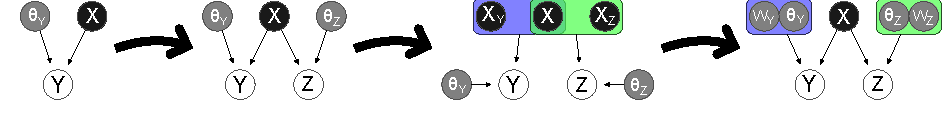
\includegraphics[width=0.9\textwidth]{bin/graphicalmodel.pdf}
  \end{center}
  \vspace{-8pt}
  \caption{\small {\it The above figure shows the evolution of the
      topology of the GP-LVM model chronologically from left to
      right. On the far left the original model is shown, where a
      single latent variable $X$ is used to represent the
      observed data $Y$. From the original model a range of
      different models for the shared data scenario have been
      proposed. The first model made an assumption that all of the
      variance in the observations was shared. This meant that the
      model was applicable to scenarios where the aim was to align two
      different manifolds. To overcome this problem a model with
      private space was introduced. However, this factorization
      introduced further challenges when learning the model. The right
      most image shows the model we propose in this paper. By
      introducing additional hyperparameters to the model encoding the
      relevance of each dimension independently for the observation
      spaces we can automatically learn the factorization of the data.
  }}
 \label{fig:grModel}
\end{figure*}

%% \begin{figure}[ht]
%% \begin{center}
%%   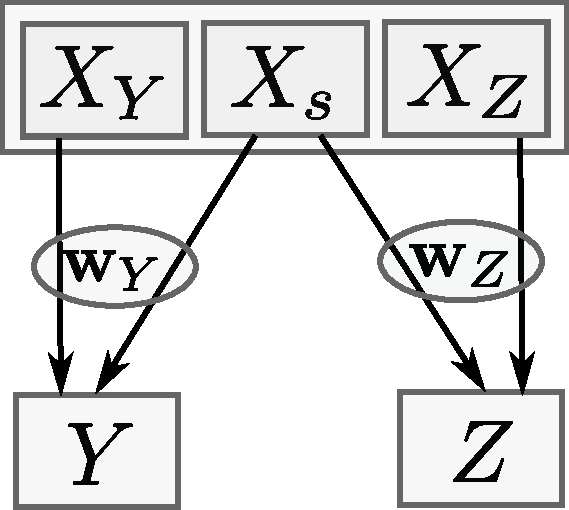
\includegraphics[width=0.18\textwidth]{../diagrams/grModel}
%% \end{center}
%% \vspace{-9pt}
%% \caption{\small{
%% .....}}
%% \label{fig:grModel}
%% \end{figure}

\par The fully Bayesian training procedure requires maximisation of
the logarithm of the joint
\emph{marginal} likelihood $p(Y,Z | \bftheta)$, where $\bftheta$ is the set of model parameters.
Although this quantity is intractable, we can invoke the variational framework of 
\cite{Titsias:bayesGPLVM10,Damianou:vgpds11} and
approximate it with a variational lower bound $\mathcal{F}_v(q,\bftheta) \approx p(Y,Z | \bftheta)$
 which relies on a variational
distribution $q(X)$. This distribution is defined in the same manner as in the \cite{Titsias:bayesGPLVM10,Damianou:vgpds11},
where it is also shown that for a single output space $Y$, the variational lower bound
breaks into two terms 
$\mathcal{L}(Y) + \text{KL}\left[ q(X) || p(X) \right]$, where the first contains
the data $Y$ and the second only involves the prior on $X$. The variational distribution $q(X)$
``binds'' the two terms together. Exploiting this observation for our model, which jointly learns
a common (factorised) latent space, allows us to write:
\begin{equation}
\mathcal{F}_v(q,\bftheta) = \mathcal{L}(Y) + \mathcal{L}(Z) + \text{KL} \left[ q(X) || p(X) \right],
\label{eq:bound}
\end{equation}
which is trivially extended for more than two observed datasets. This is
our final objective function, which is jointly maximised with respect to the model parameters (involving
the mapping parameters for $f_Y$ and $f_Z$ and the corresponding weights $\bfw_Y$ and $\bfw_Z$) and
the variational parameters.

All of the involved terms on the r.h.s of \eqref{eq:bound} are computed exactly as described in \cite{Titsias:bayesGPLVM10,Damianou:vgpds11}.
This means that, as observed in \cite{Damianou:vgpds11}, the data are only involved
in the quantities $Y Y^\T$ and $Z Z^\T$ which are $N \times N$ matrices no matter how many features
$D_Y$ and $D_Z$ are used to describe the original data. Also, these quantities are constant and can
be precomputed. Consequently, our approach is able to model datasets with millions of features.

Further, analogously to \cite{Titsias:bayesGPLVM10,Damianou:vgpds11}, the optimisation procedure simultaneously allows
the variational distribution $q(X)$ to approximate the true posterior $p(X|Y,Z)$, \ie we obtain a distribution
over the latent space. This adds extra robustness to our model, since previous approaches rely on
MAP estimates for the latent points.

%Unlike previous MAP methods, we train our model by using an approximation to the logarithm of
%the joint \textit{marginal} likelihood $\mathcal{F}_v(q, \bftheta) \approx p(Y,Z | \bftheta)$ as an objective function, where
%$\bftheta$ is the set of all model parameters and $q$ refers to the variational distribution
%which renders the approximation tractable. . We exploit the fact that in the variational
%Bayesian framework of \cite{Titsias09} the marginal likelihood $p(Y)$ of a single dataset $Y$
%breaks into two different terms 
%.... \textcolor{red}{bound, training etc.}

%$\mathcal{L}(Y) + \text{KL(q(X)||p(X)}$, where the first includes
%the data and the second only the prior, with the link being done by a variational distribution $q(X)$}

% As shown in \cite{Titsias09}, the variatio
\subsection{Dynamical Modelling}

The model formulation described in the previous section is also covering the case
when we wish to additionally model correlations between datapoints of the same output space, \ie when
$Y$ and $Z$ are multivariate timeseries. For the dynamical scenario
we follow \cite{Damianou:vgpds11,Lawrence:hgplvm07} and choose the prior on the
 latent space to depend on the times 
$\bft \in \mathbb{R}^N$ when the observations were made. In terms of computations, this
 only affects the KL term of equation \eqref{eq:bound}, which can be calculated as described
 in \cite{Damianou:vgpds11}. With this approach, we are also allowed to 
% efficiently model multiple independent sequences which, nevertheless share some commonality. 
learn the structure of multiple correlated sequences.
This is done by learning a common latent space for all timeseries while, at the same time, ignoring
correlations between datapoints that belong to different sequences.



\subsection{Inference \label{inference}}

Given a model which is trained so as to jointly represent two output spaces $Y$ and $Z$ with
a common, but factorised input space $X$, we wish to generate a new (or infer a training) set of outputs
$Z^* \in \mathbb{R}^{N^* \times D_Z}$ given a set of (potentially partially) observed test points $Y^* \in \mathbb{R}^{N^* \times D_Y}$.
This is done in three steps. Firstly, we predict the set of latent points $X^* \in \mathbb{R}^{N^* \times Q}$
which is most likely to have generated $Y^*$. For this, we use an approximation to the posterior $p(X^*|Y^*,Y)$
as is done for the standard Bayesian GP-LVM model \cite{Titsias:bayesGPLVM10,Damianou:vgpds11} and is
similar to the variational distribution $q(X)$ learned during training.
In the second step, we find the training latent points $X_{NN}$ which are closest to $X^*$ in the \emph{shared}
latent space. 
In the third step, we find outputs $Z$ from the GP-LVM likelihood $p(Z | X_{NN})$.

\par This procedure returns the set of training points $Z$ which best match the observed test points $Y^*$.
To generate novel outputs, we have to propagate the information recovered when predicting $X^*$. 
A simple way of doing this is to replace the features of $X_{NN}$ corresponding to the shared latent space,
 with those of $X^*$. This is a reasonable idea, since the shared latent space is supposed to encode the same
 kind of information for both datasets.
 A slightly more sophisticated approach is to also exploit the continuous nature of the
 optimised weights $\bfw_Y$ and give less importance to the dimensions of $X^*$ for which $w_Y^q$ is small,
 because these features are predicted with large uncertainty (variance).
 For example, we can create a new set of latent points $\hat{X}^{*}$ so that its private dimensions match those
 of $X_{NN}$ and its shared dimensions are found by averaging  
the shared dimensions of $X^*$ and $X_{NN}$ 
 as appropriate based on $\bfw_Y$. We can then generate outputs from $p(Z^* | \hat{X}^{*})$.

%We use $C_s$ to refer to the set of indices associated with the dimensions of the latent shared subspace,
%\ie $X_s = \{ \bfx_q\}_{q \in C_s}$.
%\begin{algorithm}
%\caption{Inference for SBGPLVM}
%\label{inferenceAlgorithm}
%\begin{algorithmic}
%\STATE \textbf{Input:} $Y^* = [ \bfy_1^*, ... , \bfy_N^* ], \bfy_n^* \in \mathbb{R}^{D_Y}$
%\STATE ...
%%\REPEAT
%	%\STATE $\forall q$ find $\mathit{S_q^{(k)}}$ from equation \eqref{SFixedPointQ} with $\tilde{\boldsymbol \theta}^{(k-1)}$ being fixed.
%	%\STATE Use a gradient-based method to find
%	%    $\underset{\tilde{\boldsymbol \theta}^{(k)}}{\operatorname{max}} \mathit{F(q, \boldsymbol \theta)}$ 
%	%    from equation \eqref{boundFinal} with $\mathit{S}^{(k)}$ fixed.
%    %\STATE $k = k+1$
%%\UNTIL{convergence}
%\end{algorithmic}
%\end{algorithm}
